% To be compiled by XeLaTeX, preferably under TeX Live.
% LaTeX source for ``Yanqi Lake Lectures on Algebra'' Part III.
% Copyright 2019  李文威 (Wen-Wei Li).
% Permission is granted to copy, distribute and/or modify this
% document under the terms of the Creative Commons
% Attribution-NonCommercial 4.0 International (CC BY-NC 4.0)
% https://creativecommons.org/licenses/by-nc/4.0/

% To be included
\chapter{Going-up, going-down, gradings and filtrations}

This lecture will be less self-contained than the other ones.

\section{Going-up and going-down}
In geometry, it is often crucial to know properties of a morphism between algebraically defined geometric objects. Rephrased in terms of commutative algebra, our goal is to understand the image of $\varphi^\sharp: \Spec(B) \to \Spec(A)$ where $\varphi: A \to B$ is a given ring homomorphism.

\begin{itemize}
	\item We say the \emph{going-up} property holds for $\varphi$ if for every $\mathfrak{p} \subset \mathfrak{p}'$ in $\Spec(A)$ and $\mathfrak{q} \in \Spec(B)$ with $\varphi^\sharp(\mathfrak{q}) = \mathfrak{p}$ (and we say $\mathfrak{q}$ \emph{lies over} $\mathfrak{p}$...) there exists $\mathfrak{q}' \supset \mathfrak{q}$ lying over $\mathfrak{p}'$. \index{going-up}
	\item We say the \emph{going-down} property holds for $\varphi$ if for every $\mathfrak{p} \subset \mathfrak{p}'$ in $\Spec(A)$ and $\mathfrak{q}' \in \Spec(B)$ lying over $\mathfrak{p}'$, there exists $\mathfrak{q} \subset \mathfrak{q}'$ lying over $\mathfrak{p}$. \index{going-down}
\end{itemize}
Pictorially:
\begin{center}\begin{tikzpicture}
	\node (B) at (2.5, 2) {$B$};
	\node (P) at (0,1) {$\mathfrak{q}$};
	\node (P') at (1,2) {$\mathfrak{q}'$};
	\node (A) at (2.5, 0) {$A$};
	\node (p) at (0,-1) {$\mathfrak{p}$};
	\node (p') at (1,0) {$\mathfrak{p}'$};
	\draw (P') -- (P) -- (p) -- (p') -- (P');
\end{tikzpicture}\end{center}

\begin{lemma}[Existence of minimal over-primes]\label{prop:minimal-prime}\index{minimal prime ideal}
	Let $\mathfrak{a}$ be a proper ideal in a ring $R$. There exists a prime ideal $\mathfrak{p}$ which is minimal among all primes containing $\mathfrak{a}$. If $\mathfrak{P}$ is a prime ideal containing $\mathfrak{a}$, one can choose $\mathfrak{p} \subset \mathfrak{P}$.
\end{lemma}
\begin{proof}
	One easily reduces to the case $\mathfrak{a} = \{0\}$. We want to use Zorn's Lemma\index{Zorn's Lemma} to find a minimal prime. It boils down to show that any chain $(\mathfrak{p}_i)_{i \in I}$ of prime ideals ($I$: totally ordered set with $j > i \implies \mathfrak{p}_i \supset \mathfrak{p}_j$) has a lower bound; we assume $\mathfrak{p}_i \subset \mathfrak{P}$ when $\mathfrak{P}$ is prescribed. It suffices to show $\mathfrak{p} := \bigcap_{i \in I} \mathfrak{p}_i$ is prime: if $xy \in \mathfrak{p}$ but there exists $i$ with $x \notin \mathfrak{p}_i$, then $x \notin \mathfrak{p}_j$ whenever $j \geq i$; in this case $j \geq i \implies y \in \mathfrak{p}_j$. This entails $y \in \mathfrak{p}$.
\end{proof}

\begin{lemma}
	The going-down property for $\varphi$ is equivalent to the following: for every $\mathfrak{p} \in \Spec(A)$ with $\varphi(\mathfrak{p})B \neq B$ and any minimal over-prime $\mathfrak{q}$ of $\varphi(\mathfrak{p})B$, we have $\varphi^\sharp(\mathfrak{q}) = \mathfrak{p}$.
\end{lemma}
\begin{proof}
	Assuming going-down for $\varphi$, let $\mathfrak{p}, \mathfrak{q}$ be as above. Evidently $\varphi^\sharp(\mathfrak{q}) \supset \varphi^{-1}(\varphi(\mathfrak{p})B) \supset \mathfrak{p}$. If we have $\supsetneq$, then going-down guarantees the existence of $\mathfrak{q}^\flat \subsetneq \mathfrak{q}$ lying over $\mathfrak{p}$. Thus $\varphi^{-1}(\mathfrak{q}^\flat) = \mathfrak{p}$ implies $\mathfrak{q}^\flat \supset \varphi(\mathfrak{p})B$, contradicting the minimality of $\mathfrak{q}$.
	
	To show the converse, consider $\mathfrak{p} \subset \mathfrak{p}'$ with $\mathfrak{q}'$ lying over $\mathfrak{p}'$. We have $\varphi(\mathfrak{p})B \subset \varphi(\mathfrak{p}')B \subset \mathfrak{q}' \neq B$. Take $\mathfrak{q}$ to be a minimal over-prime of $\varphi(\mathfrak{p})B$ (which exists by Lemma \ref{prop:minimal-prime}) to verify the going-down property.
\end{proof}

\begin{theorem}\label{prop:going-down-flat}
	Going-down holds for flat $\varphi: A \to B$.
\end{theorem}
\begin{proof}
	Consider $\mathfrak{p} \subset \mathfrak{p}'$ and $\mathfrak{q}'$ lying over $\mathfrak{p}'$ in the setting of going-down. First, $B_{\mathfrak{q}'}$ is flat over $A_{\mathfrak{p}'}$ by Proposition \ref{prop:flatness-localized}. Secondly, $A_{\mathfrak{p}'} \to B_{\mathfrak{q}'}$ is faithfully flat since it is local by Theorem \ref{prop:faithfully-flat-criterion} (iii), therefore induces a surjection on spectra. Take any prime of $B_{\mathfrak{q}'}$ mapping to $\mathfrak{p}A_{\mathfrak{p}} \in \Spec(A_{\mathfrak{p}'})$ and to $\mathfrak{q} \in \Spec(B)$. In view of the commutative diagrams
	\[\begin{tikzcd}
		B \arrow[r] & B_{\mathfrak{q}'} \\
		A \arrow[u, "\varphi"] \arrow[r] & A_{\mathfrak{p}'} \arrow[u, "\varphi_{\mathfrak{p}'}"']
	\end{tikzcd} \qquad \begin{tikzcd}
		\Spec(B) \arrow[d, "\varphi^\sharp"'] & \Spec(B_{\mathfrak{q}'}) \arrow[d, "\varphi_{\mathfrak{p}'}^\sharp"] \arrow[hookrightarrow, l] \\
		\Spec(A) & \Spec(A_{\mathfrak{p}'}) \arrow[hookrightarrow, l]
	\end{tikzcd}\]
	we see $\mathfrak{q}$ is the required prime in going-down.
\end{proof}

\begin{theorem}[Krull--Cohen--Seidenberg]\label{prop:Cohen-Seidenberg}
	Suppose the ring $B$ is integral over its subring $A$. The following holds.
	\begin{enumerate}[(i)]
		\item The map $\Spec(B) \to \Spec(A)$ given by $\mathfrak{q} \mapsto \mathfrak{q} \cap A$ is surjective.
		\item There are no inclusion relations in any fiber of $\Spec(B) \to \Spec(A)$.
		\item Going-up holds for $A \hookrightarrow B$.
		\item If $A$ is a local ring and $\mathfrak{p} \in \MaxSpec(A)$, then the fiber $\{ \mathfrak{q} : \mathfrak{q} \cap A = \mathfrak{p} \}$ equals $\MaxSpec(B)$.
		\item Assume $A,B$ are domains and $A$ is normal. Then going-down holds for $A \hookrightarrow B$.
		\item Assume furthermore that $B$ is the integral closure of $A$ in a normal field extension $L \supset K := \mathrm{Frac}(A)$, then $\Gamma := \mathrm{Aut}(L/K)$ acts transitively on each fiber of $\Spec(B) \to \Spec
		(A)$.
	\end{enumerate}
\end{theorem}
The last assertion should be familiar to readers with a background in algebraic number theory.
\begin{proof}
	(iv): Let $\mathfrak{q} \in \MaxSpec(B)$ and $\mathfrak{p}_0 := \mathfrak{q} \cap A$. We know $B/\mathfrak{q}$ is a field, integral over its subring $A/\mathfrak{p}_0$. We claim that $A/\mathfrak{p}_0$ is also a field, therefore $\mathfrak{p}_0 = \mathfrak{p}$. Let $x \in A/\mathfrak{p}_0 \smallsetminus \{0\}$. Its inverse in $B/\mathfrak{q}$ satisfies an integral relation $(\frac{1}{x})^n + a_{n-1} (\frac{1}{x})^{n-1} + \cdots + a_0 = 0$ over $A/\mathfrak{p}_0$. Multiplying both sides by $x^{n-1}$ yields $\frac{1}{x} \in (A/\mathfrak{p}_0)[x]$.
	
	Conversely, we have to show any $\mathfrak{q} \in \Spec(B)$ with $\mathfrak{q} \cap A = \mathfrak{p}$ is maximal. Again, there is an integral extension of domains $A/\mathfrak{p} \hookrightarrow B/\mathfrak{q}$. Consider $y \in B/\mathfrak{q}$ satisfying $y^n + a_{n-1} y^{n-1} + \cdots + a_0 = 0$, with the smallest possible $n$. If $y \neq 0$ then $a_0 \neq 0$. Since $A/\mathfrak{p}$ is a field, the recipe to produce $y^{-1} \in (A/\mathfrak{p})[y]$ is well-known.
	
	(i), (ii): Fix $\mathfrak{p}$ and consider the inclusion $A_{\mathfrak{p}} \hookrightarrow B_{\mathfrak{p}} = B \dotimes{A} A_{\mathfrak{p}}$ which is still integral (note that $A \smallsetminus \mathfrak{p}$ is a multiplicative subset of $B$, and $B_{\mathfrak{p}}$ is nonzero). We are reduced to the case $A$ is local with maximal ideal $\mathfrak{p}$. By (iv) the fiber of $\mathfrak{p}$ in $\Spec(B)$ is nothing but $\MaxSpec(B)$. This establishes (i) and (ii) since there are no inclusions among maximal ideals.
	
	(iii): Consider $\mathfrak{p} \subset \mathfrak{p}'$ and $\mathfrak{q}$ over $\mathfrak{p}$ in the setting of going-up. Then (i) is applicable to $A/\mathfrak{p} \hookrightarrow B/\mathfrak{q}$ and yields the required $\mathfrak{q}' \in \Spec(B/\mathfrak{q}) \hookrightarrow \Spec(B)$.
	
	(vi): Observe that every $\sigma \in \Gamma$ induces an $A$-automorphism of $B$. Let $K' := L^\Gamma$. By (infinite) Galois theory we know $L/K'$ is Galois and $K'/K$ is purely inseparable. Let $A'$ be the integral closure of $A$ in $K'$. First observe that 
	\[ \Spec(A') \longrightarrow \Spec(A), \quad \mathfrak{p}' \mapsto \mathfrak{p} = \mathfrak{p}' \cap A \]
	is a bijection. Indeed, $K' \neq K$ only when $p := \text{char}(K) > 0$, in which case the inverse is given by $\mathfrak{p}' = \left\{t \in A': t^{p^m} \in \mathfrak{p}, \; m \gg 0 \right\}$. Thus we assume henceforth that $L/K$ is Galois.
	
	Deal with the case $[L:K] < \infty$ first. Consider $\mathfrak{q}, \mathfrak{q}' \in \Spec(B)$ in the fiber over $\mathfrak{p}$. Suppose on the contrary that $\Gamma \mathfrak{q}$ does not meet $\mathfrak{q}'$, then by (ii) we have $\mathfrak{q}' \not\subset \sigma(\mathfrak{q})$ for each $\sigma \in \Gamma$. By the prime avoidance (Proposition \ref{prop:prime-avoidance}), there exists $x \in \mathfrak{q}' \smallsetminus \bigcup_\sigma \sigma(\mathfrak{q})$, since $\Gamma$ is finite. Now define the norm $y := N_{L/K}(x) \in K$, which is some positive power (namely $[L:K]_i$) of $\prod_{\sigma \in \Gamma} \sigma(x)$, hence belongs to $B$. Notice that
	\begin{compactitem}
		\item $A$ normal implies $y \in A$;
		\item $x \notin \sigma^{-1}(\mathfrak{q})$ for all $\sigma \in \Gamma$ implies $y \notin \mathfrak{p}$;
		\item however $y \in \mathfrak{q}' \cap A = \mathfrak{p}$ since $x \in \mathfrak{q}'$. Contradiction.
	\end{compactitem}
	
	Now suppose $[L:K]$ is infinite and $\mathfrak{q}, \mathfrak{q}'$ in the fiber over $\mathfrak{p}$. We need to use the Krull topology on $\Gamma$. For every finite, Galois subextension $E/K$ of $L/K$, define the set
	\[ \mathcal{T}(E) := \left\{ \sigma \in \Gamma: \sigma(\mathfrak{q} \cap E) = \mathfrak{q}' \cap E \right\}.  \]
	By the finite case we know $\mathcal{T}(E) \neq \emptyset$. Furthermore,
	\begin{compactitem}
		\item $\mathcal{T}(E)$ is closed in $\Gamma$ (it is the preimage of some subset of $\text{Gal}(E/K)$);
		\item $E' \subset E \implies \mathcal{T}(E') \supset \mathcal{T}(E)$;
		\item the intersection of all $\mathcal{T}(E)$ is nonempty (by the compactness of $\Gamma$ and the previous step).
	\end{compactitem}
	Taking $\sigma \in \bigcap_E \mathcal{T}(E)$ gives $\sigma(\mathfrak{q}) = \mathfrak{q}'$.

	(v): Define $L_0 := \text{Frac}(B)$ and $K := \text{Frac}(A)$. Then $L_0/K$ is algebraic and we may take a normal closure $L$ of $L_0$ over $K$. Let $C$ be the integral closure of $A$ (thus of $B$) in $L$. Consider the setting $\mathfrak{p} \subset \mathfrak{p}'$ and $\mathfrak{q} \cap A = \mathfrak{p}$ of going-down. Take any $\mathfrak{r} \in \Spec(C)$ mapping to $\mathfrak{p}$. By (iii) for $A \to C$ we obtain $\mathfrak{r}_1 \in \Spec(C)$ such that $\mathfrak{r}_1 \mapsto \mathfrak{p}'$ and $\mathfrak{r}_1 \supset \mathfrak{r}$. Next, take $\mathfrak{r}_2 \in \Spec(C)$ mapping to $\mathfrak{q}'$; by (vi) there exists $\sigma \in \text{Aut}(L/K)$ with $\sigma(\mathfrak{r}_1) = \mathfrak{r}_2$. One can check that $\mathfrak{q} := \sigma(\mathfrak{r}) \cap B$ is the required prime ideal. Explained pictorially:
	\begin{center}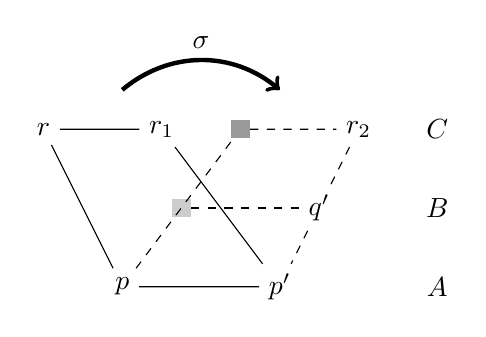
\begin{tikzpicture}
		\node (R) at (-2, 2) {$\mathfrak{r}$};
		\node (R1) at (-0.5, 2) {$\mathfrak{r}_1$};
		\node (R2) at (2, 2) {$\mathfrak{r}_2$};
		\node[fill=gray!80] (SR) at (0.5, 2) {};
		\node[fill=gray!40] (Q) at (-0.25, 1) {};
		\node (Q') at (1.5, 1) {$\mathfrak{q}'$};
		\node (P) at (-1, 0) {$\mathfrak{p}$};
		\node (P') at (1, 0) {$\mathfrak{p}'$};
		
		\node at (3, 2) {$C$}; \node at (3, 1) {$B$}; \node at (3, 0) {$A$};

		\draw (P) -- (R) -- (R1) -- (P') -- (P);
		\draw[dashed] (P) -- (SR) -- (R2) -- (Q')-- (P');
		\draw[dashed] (Q) -- (Q');
		
		\draw (-1, 2.5) edge[->, ultra thick, bend left=40] node[above, midway] {$\sigma$} (1, 2.5);
	\end{tikzpicture}\end{center}
	we first construct $\mathfrak{r}$ and then $\mathfrak{r}_1$ by going-up, then ``tilt'' it via some $\sigma$ to match $\mathfrak{r}_1$ with some chosen $\mathfrak{r}_2$ above $\mathfrak{q}'$, so that $\sigma(\mathfrak{r}) \cap B$ produces the required going-down:
\end{proof}

\begin{exercise}\label{exo:integral-closed}
	Let $A \subset B$ be an integral extension of rings. Show that $\Spec(B) \to \Spec(A)$ is a closed map (Cf.\ Proposition \ref{prop:going-up-closed}.) Hint: Let $\mathfrak{b} \subset B$ be a proper ideal, then $A/\mathfrak{b} \cap A \hookrightarrow B/\mathfrak{b}$ is still integral. Reduce the problem to showing that $V(\{0_B\}) = \Spec(B)$ has closed image in $\Spec(A)$.
\end{exercise}

\section{Subsets in the spectrum}
\begin{proposition}\label{prop:going-up-closed}
	Let $\varphi: A \to B$ be a ring homomorphism with going-up property and suppose $B$ is Noetherian. Then $\varphi^\sharp: \Spec(B) \to \Spec(A)$ is a closed map: it maps closed subsets to closed subsets.
\end{proposition}
\begin{proof}
	Consider a closed subset $V(\mathfrak{b})$ of $\Spec(B)$. First, every $\mathfrak{q} \in \Spec(B)$ with $\mathfrak{q} \supset \mathfrak{b}$ lies over a minimal over-prime of $\mathfrak{b}$, by Lemma \ref{prop:minimal-prime}. Secondly, $B$ is Noetherian implies $\text{Ass}(B/\mathfrak{b})$ is finite; in particular there are only finitely many minimal over-primes $\mathfrak{q}_1, \ldots, \mathfrak{q}_n$ of $\mathfrak{b}$.
	
	Set $\mathfrak{p}_i := \varphi^\sharp(\mathfrak{q}_i)$ for all $i$. By going-up, $V(\mathfrak{p}_i)$ is contained in $\varphi^\sharp(V(\mathfrak{b}))$. On the other hand, every $\mathfrak{p} = \varphi^\sharp(\mathfrak{q})$ with $\mathfrak{q} \in V(\mathfrak{b})$ lies over some $\mathfrak{p}_i = \varphi^\sharp(\mathfrak{q}_i)$ by the foregoing discussion. This shows $\varphi^\sharp(V(\mathfrak{b})) = \bigcup_{i=1}^n V(\mathfrak{p}_i)$ is closed.
\end{proof}

\begin{corollary}
	Suppose $B$ is Noetherian and integral over a subring $A$. Then $\Spec(B) \to \Spec(A)$ is a closed surjection with finite fibers.
\end{corollary}
\begin{proof}
	Apply Theorem \ref{prop:Cohen-Seidenberg} with Proposition \ref{prop:going-up-closed} to show that $\Spec(B) \to \Spec(A)$ is closed and surjective.

	To show the finiteness of the fiber over $\mathfrak{p} \in \Spec(A)$, note that the preimage of $V(\mathfrak{p})$ in $\Spec(B)$ equals $V(\mathfrak{p}B)$. Since there are no inclusions in the fiber over $\mathfrak{p}$, every element in that fiber must be a minimal over-prime of $\mathfrak{p}B$. We have seen in the proof of Proposition \ref{prop:going-up-closed} that there are only finitely many such minimal-over primes.
\end{proof}

Note that the ``closed surjection'' part applies to any integral extension of rings. See Exercise \ref{exo:integral-closed}.

In order to obtain further results of this type, we have to introduce more notions. Let $R$ be a ring.
\begin{definition}
	For $\mathfrak{p}, \mathfrak{p}' \in \Spec(R)$ satisfying $\mathfrak{p} \subset \mathfrak{p}'$, we say $\mathfrak{p}$ is a \emph{generalization} of $\mathfrak{p}'$, and $\mathfrak{p}'$ is a \emph{specialization} of $\mathfrak{p}$.
\end{definition}
To make geometric meaning from it, being ``specialized'' signifies that there are ``more equations'' in $\mathfrak{p}'$, therefore it corresponds a smaller embedded geometric object. For example, in $R=\CC[X,Y]$ the prime ideal $(X,Y)$ is a specialization of $(X)$, as the origin $X=Y=0$ belongs to the line $X=0$.

\begin{lemma}
	With respect to the Zariski topology, $\mathfrak{p}$ is a generalization of $\mathfrak{p}'$ if and only if $\mathfrak{p}' \in \overline{\{\mathfrak{p}\}}$.
\end{lemma}
\begin{proof}
	The condition $\mathfrak{p}' \in \overline{\{\mathfrak{p}\}}$ means that for every ideal $\mathfrak{a}$, if $\mathfrak{p} \supset \mathfrak{a}$ then $\mathfrak{p}' \supset \mathfrak{a}$. Taking $\mathfrak{a} = \mathfrak{p}$ yields $\mathfrak{p}' \supset \mathfrak{p}$, and the converse is even easier.
\end{proof}
A subset is called stable under specialization (resp. generalization) if the specialization (resp. generalization) of any member still belongs to that set. The following is straightforward.

\begin{lemma}\label{prop:stability-vs-closeness-0}
	Any closed subset is stable under specialization; any open subset is stable under generalization.
\end{lemma}

\begin{definition}\index{constructible subset}
	Suppose $R$ is Noetherian. A subset is called \emph{locally closed} if it is the intersection of an open with a closed subset, called \emph{constructible} if it is a finite union of locally closed subsets. % A possibly infinite intersection (resp. union) of constructible subsets is called \emph{pro-constructible} (resp. \emph{ind-constructible}).

	Closed subsets of the form $V(\mathfrak{p})$, where $\mathfrak{p} \in \Spec(R)$, are called \emph{irreducible}; in this case we call $\mathfrak{p}$ the \emph{generic point} of $Z$, which is uniquely characterized as the point which generalizes every member of $Z$.
\end{definition}
\begin{itemize}
	\item The foregoing definition is standard only for $R$ Noetherian. The general definition in EGA differs.
	\item These notions can be applied to any topological space $X$. In practice one usually suppose $X$ to be
		\begin{compactitem}
			\item \emph{Noetherian}: the closed subsets satisfy descending chain condition,
			\item \emph{sober}: every irreducible has a generic point,
		\end{compactitem}
		in order to get interesting results. This explains our Noetherian assumption.
	\item If $\Bbbk$ is algebraically closed, $R = \Bbbk[X_1, \ldots, X_n]/\mathfrak{a}$ corresponds to an affine algebraic variety $\mathcal{X} \subset \Bbbk^n$ and we work with $\MaxSpec(R)$ instead of $\Spec(R)$, then a subset $E \subset \mathcal{X}$ being locally closed means that it can be defined by a formula using the usual language of algebraic operations over $\CC$, with coordinate variables $X_1, \ldots, X_n$  and the symbols $=, \neq$, but \emph{without using the quantifiers $\exists, \forall$}. For example, the formula
	\[ (\neg X = 0) \vee (X = 0 \wedge Y=0) \]
	defines the constructible subset $E := \{(x,y) \in \Bbbk^2 : x \neq 0 \} \cup \{(0,0) \}$, which is neither closed nor open. Note that $E$ is the image of the polynomial map $\Bbbk^2 \to \Bbbk^2$ given by $(x,y) \mapsto (x,xy)$.
\end{itemize}

\begin{exercise}
	Show that the set of constructible subsets is stable under finite $\cup$, finite $\cap$ and taking complements.
\end{exercise}

\begin{exercise}
	Show that irreducible closed subsets $Z$ admit the following topological characterization: if $X = A \cup B$ with $A,B$ closed, then either $X=A$ or $X=B$.
\end{exercise}

Suppose $R$ is Noetherian. Given any closed subset $Z \subset \Spec(R)$, we may write $Z = Z_1 \cup \cdots \cup Z_n$ with each $Z_i$ irreducible. One way to do this is to use the primary decomposition for $\mathfrak{a}$, where we assume $Z = V(\mathfrak{a})$; then $Z_1, \ldots, Z_n$ will correspond to the minimal elements in $\text{Ass}(R/\mathfrak{a})$. One can show by purely topological means that such an irreducible decomposition is unique if we require $i \neq j \implies Z_i \not\subset Z_j$. See \cite[I.1.5]{Har77}.

\begin{lemma}\label{prop:char-constructible}
	Let $E$ be a subset of $\Spec(R)$ where $R$ is a Noetherian ring. The following are equivalent:
	\begin{enumerate}[(i)]
		\item $E$ is constructible;
		\item for every irreducible subset $Z$ of $\Spec(R)$, either $Z \cap E$ is not dense in $Z$ or $Z \cap E$ contains a nonempty open subset of $Z$.
	\end{enumerate}
\end{lemma}
\begin{proof}
	Omitted. See \cite[(6.C)]{Mat80}.
\end{proof}

\begin{theorem}[C.\ Chevalley]\label{prop:Chevalley}\index{Chevalley's theorem}
	Let $\varphi: A \to B$ be a ring homomorphism such that $A$ is Noetherian and $B$ is a finitely generated $A$-algebra. Then $\varphi^\sharp$ maps constructible subsets to constructible subsets.
\end{theorem}
\begin{proof}
	Omitted. See \cite[(6.E)]{Mat80}.
\end{proof}

Now we can give a partial converse to Lemma \ref{prop:stability-vs-closeness-0}, albeit not in the strongest form.
\begin{proposition}
	Suppose $R$ is Noetherian and $E$ is a constructible subset of $\Spec(R)$. If $E$ is stable under specialization (resp. generalization), then $E$ is closed (resp. open) in $\Spec(R)$.
\end{proposition}
\begin{proof}
	It suffices to treat the specialization-stable case by taking complements. Write the Zariski-closure $\bar{E}$ as a finite union of irreducibles components $Z$, without inclusion relations. For each irreducible component $Z$, notice that $Z \cap E$ is dense in $Z$ for all $Z$, since otherwise $\bar{E} = \overline{\bigcup_Z (Z \cap E)} = \bigcup_Z \overline{Z \cap E}$ would lead to another irreducible decomposition. Thus $Z \cap E$ contains a nonempty open of $Z$ by Lemma \ref{prop:char-constructible}. This open subset of $E$ must contain the generic point of $Z$. As $E$ is stable under specialization, we obtain $Z \subset E$. This being true for all $Z$, we deduce that $E = \bar{E}$.
\end{proof}

\begin{proposition}
	Consider a ring homomorphism $\varphi: A \to B$ satisfying going-down. Suppose $A$ is Noetherian and $B$ is a finitely generated $A$-algebra, then $\varphi^\sharp: \Spec(B) \to \Spec(A)$ is an open map.
\end{proposition}
\begin{proof}
	Let $U = \Spec(B) \smallsetminus V(\mathfrak{a})$ be an open subset. Going-down implies that $\varphi^\sharp(U)$ is stable under generalization. It suffices to show $\varphi^\sharp(U)$ is constructible, and this is the content of Chevalley's Theorem \ref{prop:Chevalley}.
\end{proof}

\section{Graded rings and modules}
Let $(\Gamma, +)$ be a commutative monoid. In most cases we consider $\Gamma = \Z_{\geq 0}$.

\begin{definition}\index{graded}
	A $\Gamma$-graded ring is a ring $R$ whose underlying additive group is endowed with a decomposition $R = \bigoplus_{\gamma \in \Gamma} R_\gamma$, such that $R_\gamma R_\eta \subset R_{\gamma + \eta}$ for all $\gamma, \eta \in \Gamma$.
	
	For $R$ as above, a $\Gamma$-graded $R$-module is an $R$-module $M$ whose underlying additive group decomposes as $M = \bigoplus_{\gamma \in \Gamma} M_\gamma$, such that $R_\gamma M_\eta \subset M_{\gamma + \eta}$ for all $\gamma, \eta \in \Gamma$; in particular, $R$ itself is a $\Gamma$-graded $R$-module. If $x \in M_\gamma \smallsetminus \{0\}$, we say $x$ is homogeneous of degree $\gamma$.\index{homogeneous}
\end{definition}
We will often omit $\Gamma$ when there is no worry of confusion. Note that if $0$ is allowed to be homogeneous, as people sometimes do, it will be homogeneous of any degree.

\begin{exercise}
	Show that in a graded ring $R$ we always have $1 \in R_0$, provides that $(\Gamma, +)$ satisfies the cancellation law: $\gamma+\eta=\eta \iff \gamma=0$. Hint: let $e_0$ be the component of $1_R$ in degree 0, argue that $x e_0 = x = e_0 x$ for all homogeneous $x \in R$. The condition $1 \in R_0$ is sometimes built into the definition of graded rings.
\end{exercise}

\begin{definition}
	A graded submodule of a graded $R$-module $M$ is a submodule $N$ with $N = \bigoplus_\gamma (N \cap M_\gamma)$, which gives rise to a natural grading $N_\gamma := N \cap M_\gamma$ on $N$.
\end{definition}
For graded $N \subset M$, the quotient $R$-module $M/N = \bigoplus_\gamma M_\gamma/N_\gamma$ is again graded. As a special case, we have the notion of graded ideals of $R$ (also known as \emph{homogeneous ideals}), and the quotient ring $R/\mathfrak{a}$ with respect to graded $\mathfrak{a}$ inherits the evident grading.

Let $N$ be an $R$-submodule of $M$ and suppose $M$ is graded. The following are easily seen to be equivalent:
\begin{enumerate}[(i)]
	\item $N \subset M$ is graded;
	\item $N$ is generated by homogeneous elements;
	\item if $x = \sum_\gamma x_\gamma \in N$ with each $x_\gamma$ homogeneous of degree $\gamma$, then $\forall \; x_\gamma \in N$.
\end{enumerate}

\begin{example}
	Let $A$ be a ring and $R := A[X_1, \ldots, X_n]$. Then $R$ is naturally $\Z_{\geq 0}$-graded by degrees: for each $d \in \Z_{\geq 0}$, let $R_d$ be the set of homogeneous polynomials of total degree $d$. Ideals generated by homogeneous polynomials are precisely the graded ideals. The importance of this grading comes from projective algebraic geometry.

	On the other hand, $R$ can also be graded by monomials by taking $\Gamma = \Z_{\geq 0} \times \cdots \times \Z_{\geq 0}$ ($n$ copies), and we set $R_{(d_1, \ldots, d_n)} = A \cdot X_1^{d_1} \cdots X_n^{d_n}$
\end{example}

Many constructions in commutative algebra can be generalized to the graded case. Let us illustrate what one can do in an important case, the primary decomposition (cf.\ \cite[\S 3.5 and Exercise 3.5]{Eis95}). In the $\Z$-graded context, it says that for a finitely generated graded module $M$ over a Noetherian graded ring, the associated primes of $M$ are all graded ideals, and one can write $\{0\} = N_1 \cap \cdots \cap N_m$ where $N_i \subset M$ are graded submodules with $\text{Ass}(M/N_i) = \{\mathfrak{p}_i\}$, $\mathfrak{p}_i \in \text{Ass}(M)$, etc. Most of the arguments in the ungraded case carry over verbatim, and the only new technique is the following

\begin{lemma}
	Let $M$ be a $\Z$-graded module over a $\Z$-graded ring $R$. If $x \in M$ and $\mathfrak{p} := \mathrm{ann}(x)$ is a prime ideal, then
	\begin{enumerate}[(i)]
		\item $\mathfrak{p}$ is a homogeneous ideal, and
		\item $\mathfrak{p} = \mathrm{ann}(y)$ for some homogeneous element $y \in M$.
	\end{enumerate}
\end{lemma}
\begin{proof}
	We begin with (i). Let $t \in \mathfrak{p}$ and $x \in M$ be such that $\mathfrak{p} = \text{ann}(M)$. Write
	\[ t = \sum_{\gamma \in \mathcal{A}} t_\gamma, \quad x = \sum_{\eta \in \mathcal{B}} x_\eta, \]
	where $t_\gamma \in R_\gamma \smallsetminus \{0\}$ and $x_\eta \in M_\eta \smallsetminus \{0\}$ for all $\gamma, \eta$. Denote by $\gamma_0$ and $\eta_0$ the minimal elements in $\mathcal{A}$ and $\mathcal{B}$, respectively. Homogenity amounts to $t_\gamma \in \mathfrak{p}$ for each $\gamma \in \mathcal{A}$, and this will be done by induction on $|\mathcal{B}|$. By a further induction on $|\mathcal{A}|$, for fixed $x$ and $\mathfrak{p}$, this can be reduced to showing $t_{\gamma_0} \in \mathfrak{p}$.
	
	First of all, considerations of degrees and $tx=0$ lead to $t_{\gamma_0} x_{\eta_0} = 0$. If $x = x_{\eta_0}$ (i.e.\ $|\mathcal{B}| = 1$), we obtain $t_{\gamma_0} \in \text{ann}(x) = \mathfrak{p}$ as required. In general:
	\begin{itemize}
		\item Suppose that $\mathfrak{p} = \text{ann}(t_{\gamma_0} x)$; since the decomposition
		\[ t_{\gamma_0} x = \sum_{\substack{\eta \in \mathcal{B} \\ \eta \neq \eta_0}} t_{\gamma_0} x_\eta \]
		involves fewer homogeneous terms, $\mathfrak{p}$ is then homogeneous by our induction hypothesis on $|\mathcal{B}|$.
		\item Suppose there exists $s \in R \smallsetminus \mathfrak{p}$ such that $s(t_{\gamma_0} x) = 0$, then $st_{\gamma_0} \in \mathfrak{p}$, hence $t_{\gamma_0} \in \mathfrak{p}$. This concludes the homogeneity (i).
	\end{itemize}
	
	From the homogeneity $\mathfrak{p}$ we infer that $\mathfrak{p} \subset \text{ann}(x_\eta)$ for each $\eta \in \mathcal{B}$. Now that
	\[ \mathfrak{p} = \text{ann}(x) \supset \prod_{\eta \in \mathcal{B}} \text{ann}(x_\eta), \]
	we have $\mathfrak{p} \supset \text{ann}(x_\eta)$ for some $\eta$, hence $\mathfrak{p} = \text{ann}(x_\eta)$. Take $y = x_\eta$ to obtain (ii).
\end{proof}

\section{Filtrations}
Now turn to filtrations. We only deal with decreasing filtrations indexed by $\Z_{\geq 0}$.
\begin{definition}\index{filtration}\index{gr@$\gr_F(M)$}
	A \emph{filtration} on a ring $R$ is a descending sequence
	\[ R = F^0 R \supset F^1 R \supset F^2 R \supset \cdots \]
	of ideals such that $F^i R \cdot F^j R \subset F^{i+j} R$. Define the associated $\Z_{\geq 0}$-graded ring
	\[ \gr_F(R) := \bigoplus_{n \geq 0} \underbracket{F^n R \big/ F^{n+1} R}_{=: \gr_F^n R} \]
	whose multiplication is defined as follows: if $x \in F^n R / F^{n+1} R$ and $y \in F^m R/F^{m+1} R$, choose liftings $\tilde{x} \in F^n R$ and $\tilde{y} \in F^m R$ and define
	\[ xy := \text{the image of }\; \tilde{x}\tilde{y}\; \text{ in }\; F^{n+m} R / F^{n+m+1} R; \]
	this is readily seen to be well-defined. The multiplication of arbitrarily many homogeneous elements can be obtained in the same recipe. The datum $(R, F^\bullet R)$ is called a \emph{filtered ring},

	Given a filtered ring $R$, a \emph{filtered $R$-module} $M$ is an $R$-module $M$ equipped with a descending sequence\footnote{In view of later applications, the filtration on a module is indexed by $\Z$ instead of $\Z_{\geq 0}$.} of submodules
	\[ \cdots \supset F^i M \supset F^{i+1} M \supset \cdots, \quad i \in \Z \]
	such that $F^i R \cdot F^j M \subset F^{i+j} M$. Define the associated graded module as the $\Z$-graded $\gr_F R$-module
	\[ \gr_F(M) := \bigoplus_{n \in \Z} \underbracket{F^n M \big/ F^{n+1} M}_{=: \gr_F^i M} \]
	whose scalar multiplication is defined using liftings as above.
\end{definition}

The subscript $F$ in $\gr$ will often be omitted. To guarantee that $\gr_F(R) \neq \{0\}$, we usually impose the harmless condition
\[ R = F^0 R \supsetneq F^1 R. \]

\begin{example}\index{filtration!$\mathfrak{a}$-adic}
	Let $\mathfrak{a}$ be a proper ideal of $R$, then $F^i R := \mathfrak{a}^i$ defines a filtration on $R$, called the \emph{$\mathfrak{a}$-adic filtration}.
\end{example}

\begin{definition}\label{def:a-stable}
	Equip $R$ with the $\mathfrak{a}$-adic filtration. A filtered $R$-module $M$ is called $\mathfrak{a}$-\emph{stable} if $\mathfrak{a} \cdot F^i M = F^{i+1} M$ for $i \gg 0$.
\end{definition}
Recall that $\mathfrak{a} \cdot F^i M \subset F^{i+1} M$ holds for all $M$, which is a part of our assumption.

As an easy example, set $F^i M := \mathfrak{a}^i M$ for $i \geq 1$, and $F^{\leq 0} M := M$; this is the $\mathfrak{a}$-adic filtration on $M$, which is obviously $\mathfrak{a}$-stable.

\begin{proposition}\label{prop:gr-Noetherian}
	Suppose $\mathfrak{a}$ is a proper ideal of $R$. If $R$ is Noetherian, so is $\gr(R)$ with respect to the $\mathfrak{a}$-adic filtration. In fact $\gr(R)$ is finitely generated over $\gr^0(R)$.
\end{proposition}
\begin{proof}
	Let $x_1, \ldots, x_n$ be generators of $\mathfrak{a}$, with images $\bar{x}_i \in \mathfrak{a}/\mathfrak{a}^2$. Then $\gr(R)$ is generated by $\bar{x}_1, \ldots \bar{x}_n$ over $R/\mathfrak{a} = \gr^0 R$, which is also Noetherian. Now apply Hilbert's Basissatz.
\end{proof}

\begin{proposition}\label{prop:gr-fg}
	Let $\mathfrak{a}$ be a proper ideal of $R$ and $M$ a finitely generated $R$-module. Suppose $M$ is endowed with an $\mathfrak{a}$-stable filtration such that $F^i M$ is finitely generated for each $i$, and $F^{\leq 0} M = M$. Then $\gr(M)$ is a finitely generated $\gr(R)$-module.
\end{proposition}
\begin{proof}
	Take $n$ such that $\mathfrak{a} \cdot F^i M = F^{i+1} M$ for all $i \geq n$. Then in $\gr(M) = \bigoplus_i \gr^i M$ we have
	\[ (\mathfrak{a}/\mathfrak{a}^2) \cdot \gr^i M = \gr^{i+1} M, \quad i \geq n. \]
	Therefore it suffices to take generators from $\gr^0 M, \ldots, \gr^n M$, each of whom is finitely generated over $R/\mathfrak{a} = \gr^0 R$.
\end{proof}

\section{Theorems of Artin--Rees and Krull}\label{sec:Artin-Rees}
Conserve the conventions in the previous section on filtrations, etc.

\begin{definition}[Morphisms between filtered objects]
	Let $(A, F^\bullet A)$ and $(B, F^\bullet B)$ be filtered rings. A \emph{morphism} between them means a ring homomorphism $\varphi: A \to B$ satisfying $\varphi(F^i A) \subset F^i B$ for all $i$. Similarly, suppose $A$ is filtered and let $M, N$ be filtered $A$-modules. A morphism $M \to N$ means a homomorphism $\psi: M \to N$ of $R$-modules satisfying $\psi(F^i M) \subset F^i N$ for all $i$.
\end{definition}
This makes the filtered rings and the filtered modules over a filtered ring into categories. Obviously, morphisms $\varphi$ between filtered objects induce graded morphisms $\gr \varphi$ between the associated graded objects. Therefore we obtain a functor from the category of filtered rings or modules into their graded avatars.

\begin{remark}
	Suppose $\varphi: M \to N$ is a morphism between filtered $A$-modules. The quotient $M/\Ker(\varphi)$ inherits a filtration from $M$, whereas the submodule $\Image(\varphi)$ inherits one from $N$. When the natural isomorphism $M/\Ker(\varphi) \to \Image(\varphi)$ is an isomorphism between filtered modules, or equivalently
	\[ \forall i \in \Z, \; \varphi(F^i M) = \varphi(M) \cap F^i N, \]
	we say $\varphi$ is a \emph{strict morphism}.
\end{remark}

It is often useful to relate properties of a filtered module or morphism to its graded counterpart. Propositions \ref{prop:gr-Noetherian} and \ref{prop:gr-fg} are such examples. Here is an example for the other direction. We say that a filtration on $M$ is \emph{exhaustive} if $\bigcup_i F^i M = M$, \emph{separating} (or \emph{Hausdorff}) if $\bigcap_i F^i M = \{0\}$

\begin{proposition}\label{prop:gr-injective}
	Suppose that $\varphi: M \to N$ is a morphism between filtered $R$-modules. If $M$ is exhaustive and separating, and $\gr\varphi$ is injective, then $\varphi$ is also injective.
\end{proposition}
\begin{proof}
	Let $x \in \Ker(\varphi)$. There exists $n$ such that $x \in F^n M$. Regard $x + F^{n+1} M$ as an element of $\gr^n M$. Then $\gr(\varphi)(x + F^{n+1} M) = \varphi(x) + F^{n+1} N = 0$, so $x \in F^{n+1} M$. Iterating this argument, we have $x \in \bigcap_{k \geq n} F^k M = \{0\}$.
\end{proof}
See Lemma \ref{prop:gr-surjective} for the case of surjections.

In what follows, $\mathfrak{a}$ always denotes a proper ideal of a ring $R$.

\begin{definition}[Blow-up algebras and modules]\index{blow-up algebra}
	Introduce an indeterminate $X$ and define the $\Z_{\geq 0}$-graded $R$-algebra
	\[ \text{Bl}_{\mathfrak{a}} R := \bigoplus_{n \geq 0} \mathfrak{a}^n X^n \; \subset R[X]. \]
	If an $R$-module $M$ is endowed with a filtration $(F^i M)_{i \geq 0}$ compatible with $\mathfrak{a}$, we define
	\[ \text{Bl}(M) := \bigoplus_{n \geq 0} (F^n M) \otimes X^n \subset M \dotimes{R} R[X]. \]
	Clearly, $\text{Bl}(M)$ is a graded $\text{Bl}_{\mathfrak{a}} R$-module.
\end{definition}

\begin{remark}
	The indeterminate $X$ is somehow a placeholder. Enlarge $\text{Bl}_{\mathfrak{a}} R$ to $\tilde{B}$ by setting the negative graded pieces to be $R \cdot X^{< 0}$, and set $T = X^{-1}$. We see that $\tilde{B}$ is actually an $R[T]$-algebra, sometimes called the \emph{Rees algebra} of $\mathfrak{a}$. Under the specialization $T=0$ we get \index{Rees algebra}
	\[ \frac{ \tilde{B}}{T \tilde{B}} \simeq \bigoplus_{n \geq 0} \frac{\mathfrak{a}^n}{\mathfrak{a}^{n+1}} \cdot T^{-n} \simeq \gr(R). \]
	On the other hand, inverting $T$ yields
	\[ \tilde{B}[T^{-1}] = \bigoplus_{n \in \Z} R \cdot T^{-n} = R[T^{\pm 1}]. \]
	This reflects a well-known deformation construction in geometry; $\gr(R)$ is actually the graded $R$-algebra corresponding to the \emph{normal cone} defined by $\mathfrak{a} \subset R$. We refer to \cite[\S 5.1]{Fu98} for details.
\end{remark}

\begin{lemma}\label{prop:Bl-fg}
	Consider a ring $R$ with proper ideal $\mathfrak{a}$, together with a filtered $R$-module $M$, assume furthermore that each $F^i M$ is finitely generated over $R$. The following are equivalent:
	\begin{enumerate}[(i)]
		\item $\mathrm{Bl}(M)$ is finitely generated over $\mathrm{Bl}_{\mathfrak{a}} R$;
		\item the filtration on $M$ is $\mathfrak{a}$-stable. (Definition \ref{def:a-stable})
	\end{enumerate}
\end{lemma}
\begin{proof}
	(i) $\implies$ (ii): Choose homogeneous generators $x_1, \ldots, x_n \in \text{Bl}(M)$ with degrees $d_1, \ldots, d_n$ respectively. It is then routine to see that
	\[ i \geq \max\{d_1, \ldots, d_n \} \implies (F^{i+1} M) X^{i+1} = \mathfrak{a} X \cdot (F^i M) X^i, \]
	that is, $\mathfrak{a} \cdot F^i M = F^{i+1} M$ for these $i$.

	(ii) $\implies$ (i): Suppose $\mathfrak{a} \cdot F^i M = F^{i+1} M$ for $i \geq d$, then $\text{Bl}(M)$ is generated by $\bigoplus_{j \leq d} (F^j M) X^j$, and each $F^j M$ is finitely generated over $R = (\text{Bl}_{\mathfrak{a}} R)_0$.
\end{proof}

\begin{theorem}[Artin--Rees]\label{prop:Artin-Rees}
	Let $R$ be a Noetherian ring endowed with $\mathfrak{a}$-adic filtration. Let $M$ be a finitely generated $R$-module and $N \subset M$ an $R$-submodule. Then the filtration on $N$ induced by the $\mathfrak{a}$-adic filtration of $M$, namely $F^i N := \mathfrak{a}^i M \cap N$, is $\mathfrak{a}$-stable.
\end{theorem}
\begin{proof}
	Define $\text{Bl}(N)$ using the induced filtration $F^i N := \mathfrak{a}^i M \cap N$, which is a submodule of the finitely generated $\text{Bl}_{\mathfrak{a}} R$-module $\text{Bl}(M)$ (Lemma \ref{prop:Bl-fg}). If $\mathfrak{a} = (a_1, \ldots, a_m)$ than $\text{Bl}_{\mathfrak{a}} R = R[a_1 X, \ldots, a_m X] \subset R[X]$, hence Noetherian by Hilbert's Basissatz. We deduce that $\text{Bl}(N)$ is finitely generated over $\text{Bl}_{\mathfrak{a}} R$. In turn, this implies $F^\bullet N$ is an $\mathfrak{a}$-stable filtration on $N$ by Lemma \ref{prop:Bl-fg}.
\end{proof}

\begin{theorem}\label{prop:intersection-thm}
	For $R, \mathfrak{a}, M$ as in the previous theorem, we set $N := \bigcap_{n \geq 0} \mathfrak{a}^n M$. Then $\mathfrak{a}N = N$.
\end{theorem}
\begin{proof}
	Since the induced filtration on $N$ is $\mathfrak{a}$-stable by Theorem \ref{prop:Artin-Rees}, for $n \gg 0$ we have
	\[ N = \mathfrak{a}^n M \cap N = \mathfrak{a} \cdot (\mathfrak{a}^{n-1} M \cap N) = \mathfrak{a} N. \]
	The assertion follows.
\end{proof}

\begin{corollary}[Krull]\label{prop:Krull-intersection-rad}
	If $\mathfrak{a} \subset \mathrm{rad}(R)$, then $\bigcap_{n \geq 0} \mathfrak{a}^n M = \{0\}$ for any finitely generated $R$-module $M$. In particular $\bigcap_{n \geq 0} \mathfrak{a}^n = \{0\}$ whenever $\mathfrak{a} \subset \mathrm{rad}(R)$.
\end{corollary}
\begin{proof}
	Theorem \ref{prop:intersection-thm} together with Nakayama's lemma imply $N = \{0\}$.
\end{proof}

\begin{corollary}[Krull's Intersection Theorem]\label{prop:Krull-intersection-domain}\index{Krull's intersection theorem}
	Let $R$ be a Noetherian domain and $\mathfrak{a}$ a proper ideal. Then $\bigcap_{n \geq 0} \mathfrak{a}^n = \{0\}$.
\end{corollary}
\begin{proof}
	Define $N := \bigcap_{n \geq 0} \mathfrak{a}^n \subset R$. By Theorem \ref{prop:intersection-thm} we have $\mathfrak{a}N = N$, thus there exists $r \in \mathfrak{a}$ with $1+r \in \text{ann}(N)$ by Nakayama's Lemma (Theorem \ref{prop:NAK}). As $\mathfrak{a}$ is proper, $1+r$ cannot be zero. Since $R$ is a domain containing $N$, the only possibility is $N=\{0\}$ as asserted.
\end{proof}